% Figure: distribution of uprightness u = cos(theta_1) + cos(theta_2) for
% the two state datasets dumped by experiments/dmc_acrobot/coverage_analysis.py.
% Source: results/dmc_acrobot/coverage.json.
%
% Bucket counts (n=2000 random states, n=846 oracle-planner states):
%
%   u-bucket        random %   oracle %
%   [-2.0, -1.5)     13.6        8.3
%   [-1.5, -1.0)     23.9        7.7
%   [-1.0, -0.5)     13.8       13.6
%   [-0.5,  0.0)     13.6       11.8
%   [ 0.0, +0.5)     17.1       14.8
%   [+0.5, +1.0)     17.9       23.6
%   [+1.0, +1.5)      0.0        8.0    <-- upright regime
%   [+1.5, +2.0)      0.0       12.2    <-- near upright
%
% TD-MPC2 rollouts (from the v0.12 README block, no full bucketed dump):
%   max u = 1.439, frac(u > 1.0) = 10.6%, frac(u > 1.5) = 0.0%. Mentioned
%   in the caption rather than overlaid as a third series.
\begin{figure}[t]
  \centering
  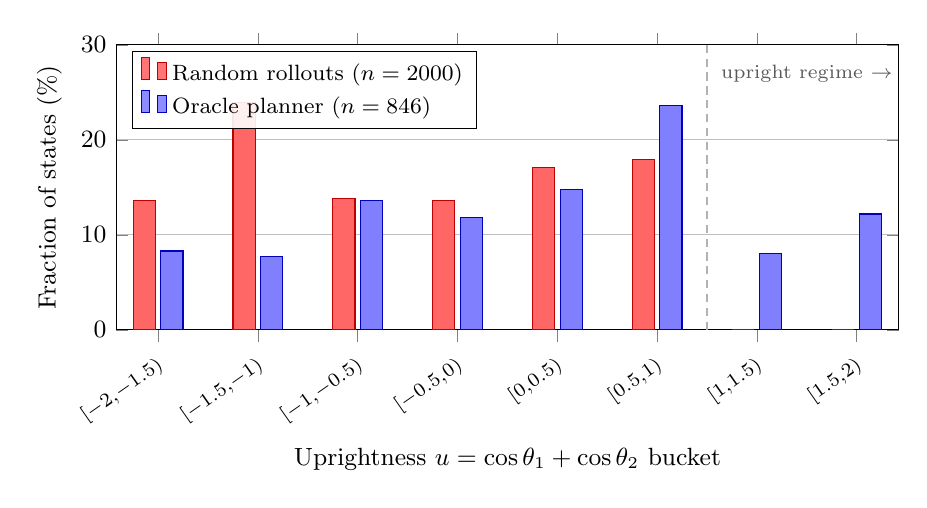
\begin{tikzpicture}
    \begin{axis}[
        width=0.95\columnwidth,
        height=5.2cm,
        font=\small,
        ybar=2pt,
        bar width=8pt,
        ymin=0, ymax=30,
        ylabel={Fraction of states (\%)},
        ymajorgrids=true,
        xtick={1,2,3,4,5,6,7,8},
        xticklabels={
          {[$-2$,$-1.5$)},
          {[$-1.5$,$-1$)},
          {[$-1$,$-0.5$)},
          {[$-0.5$,$0$)},
          {[$0$,$0.5$)},
          {[$0.5$,$1$)},
          {[$1$,$1.5$)},
          {[$1.5$,$2$)},
        },
        x tick label style={
          font=\scriptsize,
          rotate=35, anchor=north east,
        },
        xlabel={Uprightness $u = \cos\theta_1 + \cos\theta_2$ bucket},
        legend cell align=left,
        legend style={
          at={(0.02, 0.98)}, anchor=north west,
          font=\footnotesize,
          fill=white, fill opacity=0.9, draw opacity=1, text opacity=1,
        },
        enlarge x limits=0.06,
      ]
      \addplot[fill=red!60, draw=red!75!black]
        coordinates {
          (1, 13.6) (2, 23.9) (3, 13.8) (4, 13.6)
          (5, 17.1) (6, 17.9) (7, 0.0) (8, 0.0)
        };
      \addlegendentry{Random rollouts ($n = 2000$)}
      \addplot[fill=blue!50, draw=blue!75!black]
        coordinates {
          (1, 8.3) (2, 7.7) (3, 13.6) (4, 11.8)
          (5, 14.8) (6, 23.6) (7, 8.0) (8, 12.2)
        };
      \addlegendentry{Oracle planner ($n = 846$)}
      \draw[densely dashed, gray!60, thick]
        (axis cs:6.5, 0) -- (axis cs:6.5, 30);
      \node[font=\scriptsize, gray!70!black] at (axis cs:7.5, 27)
        {upright regime $\to$};
    \end{axis}
  \end{tikzpicture}
  \caption{Empirical receipt for the coverage claim. The upright regime ($u > 1$) is \emph{strictly absent} from the random-policy training data: $0/2000$ random-rollout states reach it. The oracle planner spends $20.2\%$ of its trajectory in that regime, with $12.2\%$ near upright ($u > 1.5$). TD-MPC2 rollouts (not shown; see v0.12 status) reach a maximum of $u = 1.439$ with $10.6\%$ above $u = 1$ and zero above $u = 1.5$, an intermediate coverage that still leaves the planner stuck at $0/10$ in Table~\ref{tab:robustness}. Numbers from \texttt{results/dmc\_acrobot/coverage.json}.}
  \label{fig:coverage_histogram}
\end{figure}
